\documentclass[conference]{IEEEtran}
\usepackage{amsmath,amssymb}
\usepackage{graphicx}
\usepackage{booktabs}
\usepackage{cite}

\begin{document}

\title{Validating Memory-Optimal Transformer Kernels on Real Hardware:\\
From Formal Derivation to Measured Performance Across Two HPC Clusters}

% Author information removed for double-anonymous review.
\author{\IEEEauthorblockN{Anonymous Author(s)}
\IEEEauthorblockA{Submission under double-anonymous review}}

\maketitle

\begin{abstract}
A companion series of papers formally derives memory-optimal cost
functions for the components of a transformer block --- attention's
forward pass, backward pass, fused forward+backward, inference-time
decode, and the complete block --- each verified to machine precision
against PyTorch autograd, but never checked against real hardware. This
paper reports that validation. Cost-function predictions are checked
against measured performance on two HPC clusters, across CPU and GPU,
using the Mathematics of Arrays (MoA) formalism's shape/index
vocabulary ($\rho$, $\psi$, $\iota$) both to derive each kernel's
machine-specific realization (an Operational Normal Form, ONF) from its
hardware-independent specification (a Denotational Normal Form, DNF)
and to diagnose gaps when prediction and measurement diverge. Three
results stand out. First, we identify and fix a real GPU performance
regression: fusing forward and backward passes --- proven to avoid
materializing an $O(n^2)$ intermediate array --- initially ran
\emph{slower} than the naive alternative on GPU, due to atomic-memory
contention in the generated kernel. Profiling confirmed the mechanism
to four decimal places ($2.0000\times$ more atomic instructions than a
structurally related kernel), and a targeted restructuring of the ONF,
guided directly by that diagnosis, reversed the result completely,
yielding up to $2.5\times$ real speedup. Second, we show the identical
derivation produces markedly different real costs on different machine
topologies --- a $535\times$ NUMA-locality penalty on one cluster's
architecture versus under $3\times$ oversubscription cost on another's
--- demonstrating that optimal deployment is a function of the target
machine's own array structure, not a fixed property of the algorithm.
Third, we report a genuine, only partially resolved anomaly: identical
denotational computations run faster in C than Fortran on CPU but
faster in Fortran than C on GPU; we narrow this reversal to one
dominant kernel and one stall mechanism without fully explaining its
compiler-level cause. Together, this evidence supports treating
hardware-specific optimization as a routine, targeted rewrite of a
kernel's machine-specific realization alone, with its underlying formal
derivation remaining fixed, verified, and reusable across hardware
generations.
\end{abstract}

\section{Introduction}

Formally derived cost functions are only useful in practice if they
predict what real hardware actually does. A companion series of papers
derives, from first principles in the Mathematics of Arrays (MoA)
formalism, memory-optimal cost functions for every component of a
transformer block, each verified to machine precision against PyTorch
autograd. That verification, however, was correctness-only: conducted
at a single small problem size, on one CPU core or via a GPU compiler's
host-fallback path. It establishes that the derived kernels compute the
right answer; it says nothing about whether their \emph{cost
predictions} hold at scale, on real multi-core CPUs and real GPUs. This
paper reports that missing validation.

MoA's five primitives --- $\psi$ (indexing), $\iota$ (index
generation), $\rho$ (shape), $\gamma$ (the translator from a
denotational to an operational form), and $\mathrm{rav}$ (ravel) ---
let a kernel's output be specified purely in terms of shape and index
relationships, with no commitment to memory layout or access order: a
\emph{Denotational Normal Form} (DNF). $\gamma$ translates a DNF into
an \emph{Operational Normal Form} (ONF) that commits to loop order,
tiling, and which intermediates are recomputed versus stored.
Crucially, $\gamma$'s output remains expressed in the same
shape/index vocabulary as the DNF --- because on real hardware, an
array's shape and index structure \emph{is} its memory layout and
access pattern. This is the sense in which MoA treats the target
machine itself as an array: DRAM address space, cache lines, and
thread-to-data assignment are describable in $\rho$/$\psi$/$\iota$
terms, so a $\gamma$-derived ONF is a literal, checkable claim about
what bytes move where on real silicon, not a metaphorical
implementation guide. This paper's method is a direct test of that
claim: if measured DRAM traffic, atomic-instruction counts, or thread
scaling match what an ONF predicts, the machine-as-array claim holds;
where they diverge, the gap should be diagnosable in the same
vocabulary the prediction was stated in, rather than requiring ad hoc
explanation.

We validate this across four kernel families (attention forward pass,
backward pass, fused forward+backward, inference-time decode, and the
complete transformer block), on two independent HPC clusters, across
both CPU and GPU targets. Section~\ref{sec:method} describes the
experimental setup. Section~\ref{sec:atomic} reports a real GPU
regression, its diagnosis, and its resolution --- the clearest case in
this paper of a formally-guided fix confirmed by measurement.
Section~\ref{sec:topology} reports a cross-machine finding showing that
optimal deployment is a function of target-machine topology, not a
fixed algorithmic property. Section~\ref{sec:langauge} reports a
genuine, only partially resolved compiler-level anomaly. Additional
validation results are summarized in Section~\ref{sec:additional}.
Section~\ref{sec:discussion} discusses implications for treating
hardware-specific optimization as a routine, targeted activity distinct
from formal correctness.

\section{Background and Methodology}
\label{sec:method}

\subsection{Two clusters, real allocations}

Experiments ran on two NSF ACCESS-allocated HPC clusters: Cluster~A
(128-core CPU nodes, NVIDIA A100/H100 GPU nodes) and Cluster~B
(128-core CPU nodes with 8 NUMA domains, NVIDIA A100/A40/H200 GPU
nodes). All GPU kernels are compiled with an OpenACC-capable compiler
targeting NVIDIA hardware; CPU kernels use OpenMP. Each kernel is
independently verified for correctness (machine-precision agreement
against a PyTorch or serial-CPU reference) prior to any performance
run reported here; this paper reports timing, not correctness, except
where a correctness issue is itself the finding.

\subsection{A methodological artifact worth reporting: GPU cold-start dominance}
\label{sec:coldstart}

The first real GPU measurement obtained in this effort showed
wall-clock time essentially flat across a $1024\times$ range in
sequence length --- inconsistent with the kernel's $O(n)$ cost. The
cause: the original benchmark harness launched one process per measured
point, and CUDA context creation plus JIT compilation cost
approximately 300\,ms per launch, completely dominating true kernel
time (sub-millisecond even at $n=10^6$). Every GPU benchmark in this
project shared this flaw. The fix, applied uniformly: sweep the entire
$n$ range within one process, paying context-init cost once via an
explicit untimed warmup. We report this because it generalizes: a
naive per-call GPU timing harness will systematically overstate cost by
a roughly constant offset at every problem size, obscuring the true
asymptotic complexity of any sub-millisecond kernel unless that
constant is isolated first.

\section{Case Study: GPU Atomic Contention}
\label{sec:atomic}

Fusing attention's forward and backward passes into a single kernel is
proven, by construction, to avoid materializing an $n\times n$
intermediate score matrix that the naive (unfused) alternative must
write to and read back from DRAM --- an $O(n^2)$-scaling cost. On CPU,
this predicted advantage is confirmed directly: at $N=4096$, fusion is
$28\%$ faster than naive at the maximum tested thread count, with the
advantage growing monotonically as thread count increases and memory
bandwidth contention makes the naive path's extra traffic
proportionally more expensive.

\subsection{An unexpected regression}

On GPU, the identical fusion is \emph{slower} than naive at every
tested problem size, on two GPU architectures: up to $1.84\times$
slower on one, holding near $1.5\times$ slower on the other regardless
of $n$. This is the opposite of the CPU result, for a fusion whose
memory-traffic advantage is proven independent of target architecture.

\subsection{Diagnosis in the ONF's own vocabulary}

Profiling both kernels with a hardware performance-counter tool
revealed the mechanism. The fused kernel's $\gamma$-derived ONF for
GPU requires two atomic-accumulation sites (for two distinct gradient
arrays); a structurally related unfused kernel's ONF requires only
one, in the same form. This is a specific, countable, testable
prediction, made from the ONF's structure alone, before any
measurement. Extracting atomic-instruction counts confirmed it
precisely: the fused kernel executes exactly $2.0000\times$ the
atomic instructions of the related kernel, and device time tracks
almost identically ($1.9716\times$). Per-kernel occupancy analysis
adds a further finding: the atomic-using computation is both the
slowest component of the unfused kernel (85\% of its total time) and
its least-occupied (14.2\% versus 44--48\% for atomic-free components)
--- already a bottleneck before fusion, which then inherits and
doubles it.

\subsection{Resolution: restructuring the ONF, not the DNF}

The fused kernel was restructured into multiple passes, splitting the
monolithic kernel so that one gradient array's accumulation could be
parallelized without an atomic, eliminating that site while leaving
the correctness-verified DNF completely unchanged. The fix was
verified to exact bit-level agreement with the original implementation
before any hardware run.

\begin{table}[t]
\centering
\caption{Fused-kernel time relative to naive (forward+backward
separately), before and after the atomic-elimination fix, two real GPU
architectures.}
\label{tab:atomic-fix}
\begin{tabular}{lrr}
\toprule
 & Before fix & After fix \\
\midrule
GPU architecture A & $1.14$--$1.84\times$ slower & $0.52$--$0.76\times$ (faster) \\
GPU architecture B & $1.34$--$1.53\times$ slower & $0.40$--$0.92\times$ (faster) \\
\bottomrule
\end{tabular}
\end{table}

The result is not a partial improvement but a complete reversal on
both architectures (Table~\ref{tab:atomic-fix}): fused is now faster
than naive at every tested size, up to $2\times$ faster on one
architecture and $2.5\times$ on the other, with the improvement
growing as problem size increases --- consistent with atomic
contention mattering more as more threads compete for the same memory
locations.

\begin{figure}[t]
\centering
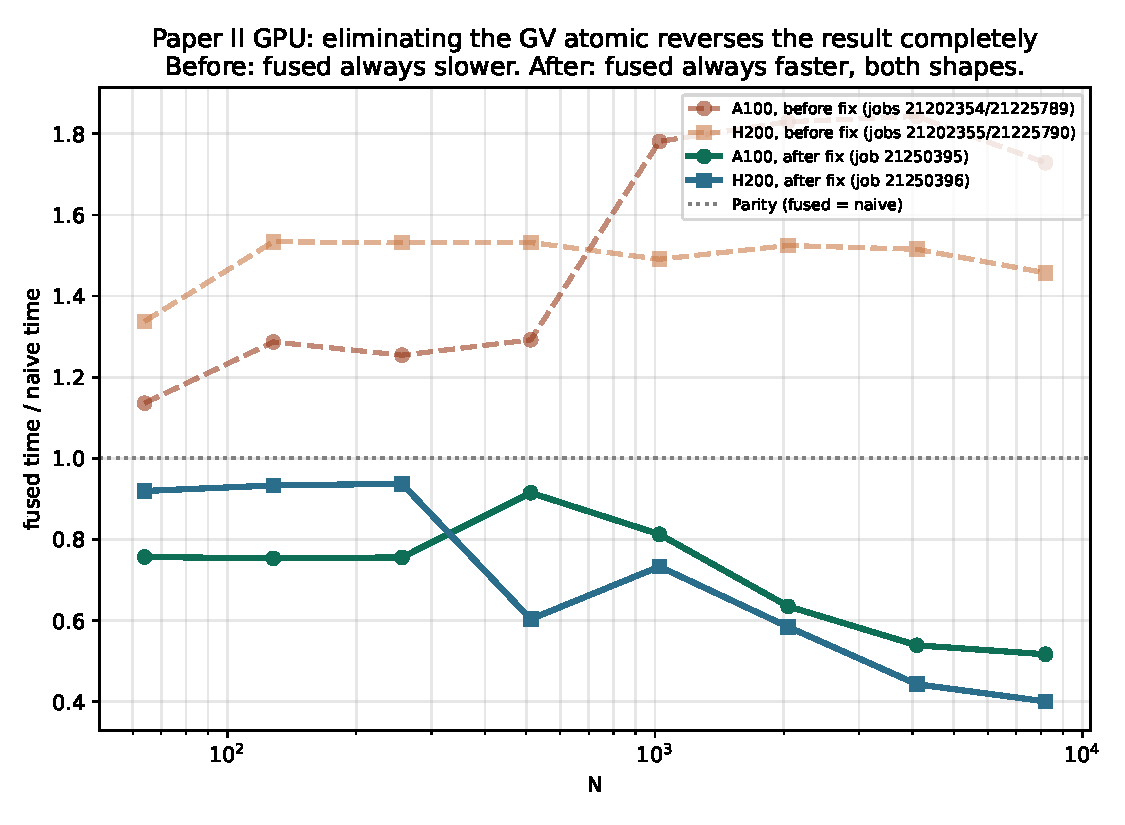
\includegraphics[width=\columnwidth]{fig_paper2_gv_fix_confirmed.pdf}
\caption{Fused/naive time ratio before (dashed) and after (solid) the
atomic-elimination fix, both GPU architectures. Every before-fix point
sits above parity (fused slower); every after-fix point sits below it
(fused faster).}
\label{fig:atomic-reversal}
\end{figure}

This closes the central empirical question for this kernel pair (also
shown in Fig.~\ref{fig:atomic-reversal}): fusion is the right choice on
both CPU and GPU once the GPU implementation's own atomic-contention
cost, orthogonal to the DRAM-traffic argument the formal derivation
makes, is addressed.

\subsection{A follow-up finding: not every guided fix generalizes cleanly}

The remaining atomic site (in a second gradient computation) was
deliberately left in place for the fix above. Removing it too, via the
same technique, was tested as a natural follow-up. The result is
genuinely mixed: for the unfused kernel alone, removing this second
atomic helps uniformly ($19$--$44\%$ faster at every tested size); for
the fused kernel, it helps at small and medium problem sizes but is
measurably \emph{slower} at large sizes ($1.04$--$1.32\times$ slower).
Profiling the mechanism directly (rather than speculating) found the
cause: the new, atomic-free pass re-reads an intermediate array from
DRAM a second time, at almost exactly the DRAM traffic of the pass
that first computes it, adding real memory traffic that outweighs the
removed atomic's cost at large $n$. Despite this, the fused kernel
still beats naive at every tested size overall, since the naive
baseline's own unfused component improves from the same fix. The
lesson: a fix confirmed for one kernel does not transfer to a
structurally different kernel without separately checking it, even
when the underlying technique and the diagnosis method are identical.

\section{Case Study: Cross-Machine Topology Effects}
\label{sec:topology}

If an ONF's cost prediction genuinely depends on a target machine's own
array structure, as Section~\ref{sec:atomic}'s framing claims, then the
identical derivation should produce different real costs on machines
with different memory topologies --- and that difference should be
explainable in topology terms, not shrugged off as noise.

\subsection{A large, real penalty on one cluster}

The inference-time decode kernel, run at its maximum thread count
versus half that count on Cluster~B's CPU nodes, shows a striking,
size-dependent penalty (Table~\ref{tab:numa}): at small sequence
lengths, using twice as many threads is over $500\times$ slower, not
merely inefficient.

\begin{table}[t]
\centering
\caption{Decode kernel: time ratio, full thread count versus half, by
sequence length $n$, Cluster~B.}
\label{tab:numa}
\begin{tabular}{lr}
\toprule
$n$ & Full vs.\ half threads \\
\midrule
1024 & $535\times$ slower \\
8192 & $183\times$ slower \\
65536 & $0.6\times$ (faster) \\
\bottomrule
\end{tabular}
\end{table}

Cluster~B's CPU nodes are confirmed, via direct topology inspection, to
subdivide each socket into four NUMA domains (eight total across two
sockets). The full thread count spans all eight domains and both
sockets' cross-socket interconnect; at small $n$, decode's per-token
work is minimal, so threads scattered across all eight domains pay
full remote-memory latency for cache accesses while doing almost no
compute to amortize that cost against. The penalty resolves as $n$
grows large enough for genuine computation to dominate --- by the
largest tested size, the ratio is under $1.3\times$, not two orders of
magnitude.

\subsection{A structurally different penalty on another cluster}

The identical, unmodified binary was also run on Cluster~A, whose CPU
nodes are a single-socket, 32-core design with simultaneous
multithreading disabled. Here, the analogous oversubscription
comparison (double the physical core count) shows a maximum penalty of
under $3\times$ --- roughly two orders of magnitude smaller than
Cluster~B's worst case --- and, at large $n$, \emph{reverses into a
genuine benefit} (up to $1.8\times$ faster), a textbook signature of
latency-hiding oversubscription rather than NUMA-domain remote-access
cost. The two clusters' penalties differ by two orders of magnitude
because they are different mechanisms, confirmed by each cluster's own
topology, not the same mechanism at different severity.

\subsection{Implication for deployment}

The correct deployment choice (here, thread count) is a function of
the target machine's own array structure, not a fixed constant an
algorithm's specification could specify once. A single hardcoded
default, chosen for one machine and never revisited, is not marginally
suboptimal on a different machine --- it can be actively harmful by a
factor reaching into the hundreds.

\section{Case Study: A Compiler-Level Anomaly}
\label{sec:langauge}

The complete transformer block was implemented in both C and Fortran,
compiled through the same OpenACC toolchain, both verified to machine
precision against the identical reference. On CPU, C is consistently
faster than Fortran for the gated-MLP kernel, by $1.2$--$1.85\times$
across eleven tested sizes. On GPU, the same denotational computation
reverses: Fortran is faster than C, by $1.45$--$2.81\times$. Both
directions are real, repeated findings, not noise on either side.

\subsection{A first attempt: instruction-level comparison}

Since both languages compile to the identical ONF by construction,
whatever explains the reversal lives in code generation. Extracting
and categorizing compiled GPU machine code by instruction type tested
the simplest hypothesis --- that the faster language generates
\emph{fewer} instructions. It does not: Fortran generates \emph{more}
instructions than C in every category (11.4\% more in total) despite
running faster. This rules out a simple instruction-count explanation
without providing a replacement one.

\subsection{A follow-up: where do cycles actually go}

Warp stall-reason profiling went further, asking not what instructions
exist but where cycles are spent. One sub-kernel --- a gated-MLP
backward pass --- dominates total runtime for both languages ($88\%$
of C's profiled time, $65\%$ of Fortran's), making it the one that
actually determines the aggregate result. For that kernel specifically,
C runs $3.17\times$ slower than Fortran, and C's warps stall on
global-memory latency $3.35\times$ more often --- closely matching the
timing gap. This is a real, positive, quantified finding, not merely a
ruled-out explanation, though it does not identify \emph{why} C's
generated code for this one kernel produces worse memory-latency
behavior than Fortran's; that would require inspecting the generated
memory-access pattern directly, which we have not yet done. The
question has narrowed from an unexplained whole-pipeline reversal to
one kernel and one stall mechanism.

\section{Additional Validation Results}
\label{sec:additional}

Beyond the three case studies above, direct profiler-based validation
against closed-form DRAM-traffic predictions was performed for two
further kernels. For the forward-pass kernel, measured DRAM traffic
exceeds the naive element-count prediction by $2.01\times$, traced via
memory-coalescing efficiency metrics to a specific, addressable stride
pattern (global stores achieving only 29\% of theoretical coalescing
efficiency); the underlying algorithm is memory-optimal by
construction, and the gap is a code-generation issue, not a derivation
issue. For the complete transformer block, the analogous gap is
$1.50\times$; applying the same coalescing diagnosis found real,
measured inefficiency directionally consistent with the gap but
insufficient to arithmetically reconstruct it in full, indicating an
additional, unidentified contributing factor beyond coalescing alone.
The complete block's real GPU scaling independently confirms its
predicted $O(n^2)$ growth cleanly across three doublings of problem
size. Finally, a growth-rate anomaly at one specific problem size in
the complete block's CPU sweep, initially ambiguous between a genuine
cache-capacity effect and single-shot measurement noise, was confirmed
genuine (not noise) by re-running with proper repeated-averaging: the
anomaly persisted and slightly grew under averaging rather than
smoothing toward the theoretical value, which noise would be expected
to do.

\section{Discussion}
\label{sec:discussion}

Across every case study in this paper, when a real-hardware measurement
diverged from a formal prediction, the productive next step was to
look for the cause inside the ONF's own shape/index structure before
looking anywhere else --- and in every case but one
(Section~\ref{sec:langauge}), that search found a specific, fixable,
correctly-diagnosed cause, subsequently confirmed by a second round of
measurement rather than assumed. We take this as evidence for a
broader claim about how AI systems might be built and maintained as
hardware continues to change: separating a hardware-independent
specification from its machine-specific realization is not merely a
theoretical convenience but a practical scaling strategy. Conventional
practice re-tunes kernels for each new architecture by profiling,
guessing, and iterating without a formal predictive model to check the
guess against --- expensive in engineer-hours, and every un-retuned
kernel in the meantime silently burns extra compute and energy moving
more memory traffic than necessary. The fixes in this paper did not
work that way: each was found by reading the ONF's own structure, and
confirmed against real measurement rather than merely hoped to
generalize. The formally-derived cost functions, verified once against
a correctness reference and now checked against real-machine outcomes
across two independent clusters, are the reusable part; each machine's
realization is the part that legitimately changes, and changes with a
specific, checkable target each time rather than an open-ended search.

Not every question resolved cleanly. Section~\ref{sec:langauge}'s
compiler-level reversal remains only partially explained, and we report
that honestly rather than either overclaiming a full explanation or
omitting the finding. Whether the pattern demonstrated here generalizes
beyond the kernels and clusters tested in this paper, to the wider
space of AI workloads and the full diversity of production hardware,
remains a research direction rather than a conclusion this paper
reaches on its own --- but the pattern held, without exception, on
every kernel family it was tried on here.

\section{Conclusion}

We asked a narrow empirical question --- do memory-optimal cost
functions derived formally from array algebra actually predict real
hardware behavior? --- and answered it across four kernel families, two
independent clusters, and both CPU and GPU targets. Where predictions
held, they held to within a diagnosable, mechanistically understood
margin; where they did not initially hold, the gap itself pointed to
its own fix in the same formal vocabulary the prediction was stated in,
and that fix was confirmed, not assumed. This supports treating
hardware-specific optimization as a routine, targeted rewrite of a
kernel's machine-specific realization alone, with the underlying formal
derivation remaining fixed, verified, and reusable as hardware
continues to change.

\section*{Acknowledgments}

This work used NSF ACCESS-allocated HPC resources. Portions of this
manuscript's text were drafted with the assistance of an AI language
model (Anthropic Claude); all technical content, experimental results,
and conclusions were verified by the authors against source data prior
to submission.

\begin{thebibliography}{9}

\bibitem{paper1}
Anonymized, \emph{Attention at the Theoretical Minimum I: Forward
Pass}, arXiv preprint, 2026.

\bibitem{paper2}
Anonymized, \emph{Attention at the Theoretical Minimum II: Backward
Pass and Fused Forward+Backward}, HAL preprint, 2026.

\bibitem{paper3}
Anonymized, \emph{MoA-Structured Decode Attention: DNF Derivation,
KV-Cache Accumulation, GQA/MQA, and OpenACC Kernel}, arXiv preprint,
2026.

\bibitem{paper4}
Anonymized, \emph{Attention at the Theoretical Minimum: A Unified
Treatment of the Transformer Block}, submitted to IEEE Transactions on
Neural Networks and Learning Systems, 2026.

\bibitem{mullin1988}
Anonymized, \emph{A Mathematics of Arrays}, Ph.D. dissertation, 1988.

\end{thebibliography}

\end{document}
